\documentclass[12pt, a4paper]{article}
\usepackage[a4paper,top=1.5cm, bottom=1.5cm, left=2cm, right=2cm]{geometry}
\usepackage{graphicx} % Required for inserting images
%%% Работа с русским языком
\usepackage{cmap}					% поиск в PDF
\usepackage{mathtext} 				% русские буквы в фомулах
\usepackage[T2A]{fontenc}			% кодировка
\usepackage[utf8]{inputenc}			% кодировка исходного текста
\usepackage[english,russian]{babel}	% локализация и переносы
\usepackage{float}
\usepackage{subcaption}
\usepackage{wrapfig}
\usepackage{tabularx}
\usepackage{multirow}

\usepackage[unicode]{hyperref}
\usepackage{xcolor}
\hypersetup{
    colorlinks=true,
    urlcolor=blue,
    linkcolor=blue,
    citecolor=blue
}
%%% Дополнительная работа с математикой
\usepackage{amsmath,amsfonts,amssymb,mathtools} % AMS
\usepackage{icomma} % "Умная" запятая: $0,2$ --- число, $0, 2$ --- перечисление
%% Номера формул
\mathtoolsset{showonlyrefs=true} % Показывать номера только у тех формул, на которые есть \eqref{} в тексте.
%% Шрифты
\usepackage{euscript}	 % Шрифт Евклид
\usepackage{mathrsfs} % Красивый матшрифт
%% Свои команды
\DeclareMathOperator{\sgn}{\mathop{sgn}}
%% Перенос знаков в формулах (по Львовскому)
\newcommand*{\hm}[1]{#1\nobreak\discretionary{}
{\hbox{$\mathsurround=0pt #1$}}{}}


\usepackage{indentfirst}
% \usepackage[italicdiff]{physics}
% \graphicspath{{images/}}
\DeclareGraphicsExtensions{.pdf,.png,.jpg}
\usepackage{enumitem}
\usepackage{caption}
\usepackage{array}
\usepackage{ragged2e}

\usepackage{tikz}
\usetikzlibrary{arrows.meta, calc, patterns, decorations.markings}

\usepackage{booktabs}

\newcommand{\diff}{\mathrm{d}}
\newcommand{\unit}[1]{\text{#1}}




\begin{document}



\include{titlepage}
\begin{titlepage}
\thispagestyle{empty}

\begin{center}
\small
Министерство науки и высшего образования Российской Федерации\\[2mm]
\textbf{ФЕДЕРАЛЬНОЕ ГОСУДАРСТВЕННОЕ АВТОНОМНОЕ
ОБРАЗОВАТЕЛЬНОЕ УЧРЕЖДЕНИЕ ВЫСШЕГО ОБРАЗОВАНИЯ}\\[1mm]
«МОСКОВСКИЙ ФИЗИКО-ТЕХНИЧЕСКИЙ ИНСТИТУТ\\
(НАЦИОНАЛЬНЫЙ ИССЛЕДОВАТЕЛЬСКИЙ УНИВЕРСИТЕТ)»\\
(МФТИ, Физтех)
\end{center}

\vspace{18mm}

\begin{center}
\large \textbf{КАФЕДРА КВАНТОВОЙ ЭЛЕКТРОНИКИ}\\[10mm]
\Large \textbf{ОТЧЁТ}\\[2mm]
\large \textbf{ПО ЛАБОРАТОРНОЙ РАБОТЕ}\\[14mm]
\Large \textbf{ЛАЗЕРНЫЙ ГИРОСКОП}
\end{center}

\vfill

% Блоки с подписями слева, линии и пояснения справа
\noindent
\begin{tabular}{@{}p{0.44\linewidth}p{0.52\linewidth}@{}}
\textit{Работу выполнили:} & Вакорина Анастасия,

Винокуров Владислав,

Выгнанчук Валерия,

Ескина Ольга,

Рагозина Елизавета,

Струков Олег,

Группа Б04-404 \\[8mm]

\textit{Работу принял, оценка:} & \\[3mm]
 \\
\end{tabular}


\vspace{12mm}

\begin{center}
\small Долгопрудный, \the\year{}~г.
\end{center}

\end{titlepage}








\newpage





\section*{Теоретическая часть}


\subsection*{Эффект Саньяка в пассивном интерферометре}
В основе работы лазерного гироскопа лежит \textit{эффект Саньяка}: во вращающемся оптическом контуре две волны, распространяющиеся из одной точки в противоположных направлениях, возвращаются в исходную точку в разные моменты времени. Рассмотрим идеальный кольцевой интерферометр радиусом $R$, вращающийся с угловой скоростью $\Omega$. Излучение в точке $A$ разделяется на две волны, после встречи в точке $A'$ они вновь объединяются.

За время обхода контура точка встречи успевает сместиться, поэтому времена прохождения волн определяются уравнением:
\begin{equation}
    c\, t_{\pm} = 2\pi R \pm \Omega R\, t_{\pm},
\end{equation}
откуда
\begin{equation}
    t_{\pm} = \frac{2\pi R}{c \mp \Omega R}.
\end{equation}
Индекс <<+>> относится к волне, бегущей по направлению вращения, <<$-$>> --- против. Разность времён обхода в первом приближении ($\Omega R \ll c$):
\begin{equation}
    \Delta t = t_{+} - t_{-} \approx \frac{4\pi R^2 \Omega}{c^2} = \frac{4S\Omega}{c^2},
\end{equation}
где $S = \pi R^2$ --- площадь, охватываемая контуром. Разность оптических путей:
\begin{equation}
    \Delta L = c\,\Delta t = \frac{4S\Omega}{c}.
\end{equation}
Это выражение справедливо для контура произвольной формы.



\subsection*{Кольцевой лазер как датчик вращения}
Пассивный интерферометр Саньяка мало пригоден для практики: при $S = 1\,\unit{м}^2$ и $\Omega = 2\pi\,\unit{рад/с}$ разность путей $\Delta L \approx 0{,}08\,\unit{мкм} \ll \lambda = 0{,}633\,\unit{мкм}$. Чувствительность кардинально повышается при помещении в контур активного элемента --- так появляется кольцевой лазер.

Частота генерации лазера определяется условием:
\begin{equation}
    \nu_m = \frac{c}{L}\,m, \quad m = 1,2,3,\ldots
\end{equation}
Во вращающемся лазере частоты встречных волн для продольной моды $m$ соответствуют разным длинам оптического пути $L_{\pm} = L \pm \Delta L$:
\begin{equation}
    \nu_{\pm} = \frac{c\,m}{L \pm \Delta L}.
\end{equation}
Разность частот генерации встречных волн:
\begin{equation}
    \Delta \nu = \nu_{+} - \nu_{-} = \frac{4S}{\lambda L}\,\Omega = K\,\Omega,
\end{equation}
где $K = \frac{4S}{\lambda L}$ --- \textit{масштабный коэффициент} гироскопа. Зависимость $\Delta \nu(\Omega) = K\,\Omega$ называется \textit{выходной характеристикой}.


\begin{figure}[H]
    \centering
    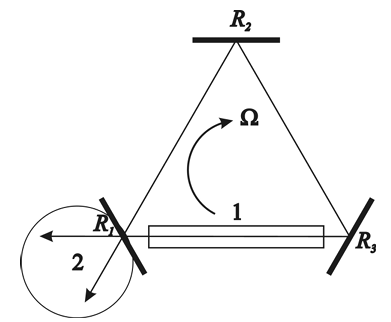
\includegraphics[width=0.4\textwidth]{1.png}
    \caption{Трёхзеркальный лазерный гироскоп: 1 --- активная среда, 
    2 --- смеситель с фотодетекторами, $R_1, R_2, R_3$ --- зеркала резонатора.}
    \label{fig:gyro_scheme}
\end{figure}





\subsection*{Регистрация сигнала и цена импульса}
Встречные волны смешиваются на оптическом смесителе. Интенсивность интерференционной картины в точке $x$:
\begin{equation}
    I(x) = I_0\left[1 + \cos\left(\frac{2\pi}{\lambda}\,\varepsilon\, x + \Delta\omega\, t + \phi_0\right)\right],
\end{equation}
где $\phi_0$ --- постоянный сдвиг фаз, $\varepsilon = 2n\,\delta\theta$ --- угол расхождения волн, $n$ --- показатель преломления призмы смесителя, $\delta\theta$ --- отклонение угла призмы от $90^\circ$, $\Delta\omega = 2\pi\,\Delta\nu$. Интерференционная картина <<бежит>> со скоростью, пропорциональной $\Omega$.

Число полос, проходящих мимо фотоприёмников за время $t$:
\begin{equation}
    N = \int_0^t \Delta \nu\,\diff t = \frac{4S}{\lambda L}\int_0^t \Omega\,\diff t = \frac{4S}{\lambda L}\,\Phi = K\,\Phi,
\end{equation}
где $\Phi$ --- полный угол поворота. Один импульс соответствует углу $\frac{\lambda L}{4S}$ --- \textit{цене импульса}.

\subsection*{Погрешности лазерного гироскопа}
Идеальная линейная характеристика искажается тремя основными эффектами: сдвигом нуля, изменением масштабного коэффициента и захватом частоты.

\textbf{Сдвиг нуля} обусловлен неравенством коэффициентов преломления для встречных волн. В газоразрядной трубке существует поток атомов при накачке постоянным током, что приводит к \textit{эффекту Физо--Френеля}. Скорость света в движущейся среде:
\begin{equation}
    c' = \frac{c}{n} \pm V\left(1 - \frac{1}{n^2}\right),
\end{equation}
где $V$ --- скорость движения среды. Разность оптических путей по и против движения среды:
\begin{equation}
    L_{\pm} = \frac{L}{c'} \cdot c = \frac{L}{\frac{c}{n} \pm V\left(1 - \frac{1}{n^2}\right)} \cdot c.
\end{equation}
Это приводит к сдвигу частоты:
\begin{equation}
    \Delta \nu \approx \frac{V}{\lambda}\left(1 - \frac{1}{n^2}\right).
\end{equation}

\textbf{Изменение масштабного коэффициента} связано с общим изменением показателя преломления активной среды (при нагреве, утечке газа) и эффектом затягивания частоты к центру контура усиления.

\subsection*{Захват частоты (синхронизация встречных волн)}
Наиболее критичная погрешность --- \textit{захват частоты}. При вращении гироскопа со скоростью ниже критического значения $\Omega_L$ (\textit{порога захвата}) частоты встречных волн синхронизируются, и $\Delta \nu = 0$. В этой <<мёртвой зоне>> измерение малых скоростей невозможно.

Явление захвата свойственно связанным автоколебательным системам. Лазерный генератор описывается уравнением, аналогичным уравнению Ван-дер-Поля:
\begin{equation}
    \frac{\diff^2 e}{\diff t^2} + \left[\gamma - g_0\left(1 - \frac{|e|^2}{e_{\text{нас}}^2}\right)\right]\frac{\diff e}{\diff t} + \omega_m^2\, e = N(t),
\end{equation}
где $e$ --- комплексная амплитуда поля, $\gamma = \frac{1}{\tau_c}$ --- потери, $g_0$ --- ненасыщенное усиление, $e_{\text{нас}}$ --- амплитуда насыщения, $\omega_m$ --- резонансная частота, $N(t)$ --- случайное возбуждение (спонтанное излучение).

Система двух связанных осцилляторов:
\begin{equation}
    \begin{cases}
        \ddot{e}_1 + \lambda_1 \dot{e}_1 + \omega_{01}^2\, e_1 = \Theta_1\, e_2, \\
        \ddot{e}_2 + \lambda_2 \dot{e}_2 + \omega_{02}^2\, e_2 = \Theta_2\, e_1,
    \end{cases}
\end{equation}
где $\Theta_{1,2}$ --- коэффициенты связи, обусловленные обратным рассеянием на зеркалах.

Основной источник связи --- взаимное обратное рассеяние волн на неоднородностях зеркал. С учётом эффективного обратного рассеяния уравнение для фазы $\Psi$ между волнами:
\begin{equation}
    \dot{\Psi} = \Omega' - \Omega_L\,\sin(\Psi + \beta),
\end{equation}
где $\Omega'$ --- частота биений без связи, $\beta$ --- постоянный фазовый угол обратного рассеяния, $\Omega_L = \frac{r\,c}{L}\,\frac{E_2}{E_1}$ --- порог захвата.

При $\Omega' < \Omega_L$ встречные волны синхронизированы ($\Delta \nu = 0$). При $\Omega' > \Omega_L$ эффективная разность частот:
\begin{equation}
    \Omega_b = \sqrt{(\Omega')^2 - \Omega_L^2}.
\end{equation}
Таким образом, эффективная разность частот меньше разности при отсутствии связи.

\subsection*{Оценка области синхронизации}
Коэффициент рассеяния зеркала $R_s = 0{,}1\%$ (по амплитуде). Доля амплитуды, рассеиваемой в противоположном направлении:
\begin{equation}
    r \approx R_s\,\frac{\lambda}{\pi\,\omega_0} \approx 7{,}6 \cdot 10^{-7}.
\end{equation}
Для параметров гироскопа $L = 20\,\unit{см}$, $S = 25\,\unit{см}^2$, $\lambda = 632{,}991\,\unit{нм}$ масштабный коэффициент $K = 1378{,}6\,\unit{град}^{-1}$. Область синхронизации:
\begin{equation}
    \Omega_L \approx 1139{,}7\,\unit{рад/с} \quad (\approx 473{,}7\,\unit{град/ч}).
\end{equation}
Для сравнения: угловая скорость вращения Земли $\approx 15\,\unit{град/ч}$, вертикальная составляющая на широте МФТИ ($55^\circ 55' 43''$) --- $12{,}4\,\unit{град/ч}$. Таким образом, без частотной подставки измерение скорости вращения Земли невозможно.

\subsection*{Зеемановская частотная подставка}
Для вывода рабочей точки из зоны захвата создаётся дополнительная разность частот --- \textit{частотная подставка}. В данном макете используется \textit{эффект Зеемана}.

При наложении продольного магнитного поля $H$ контур усиления расщепляется на два компонента для волн с правой и левой круговой поляризацией:
\begin{equation}
    \Delta \nu_z = \pm \frac{g\,\mu_B}{h}\,H,
\end{equation}
где $g = 1{,}3$ --- множитель Ланде, $\mu_B = 9{,}27 \cdot 10^{-24}\,\unit{Дж/Тл}$ --- магнетон Бора.

Ключевую роль играет \textit{аномальная дисперсия} активной среды с инверсией населённостей. Показатель преломления $n$ зависит от частоты: для мод с частотами ниже центральной $n$ уменьшается (резонансные частоты растут), для частот выше центральной --- $n$ увеличивается (резонансные частоты уменьшаются). Каждая встречная волна затягивается к центру \textit{своего} расщеплённого контура.

Отстройка частоты генерации от собственной частоты:
\begin{equation}
    \nu - \nu_r = \frac{G_0}{k}\,\frac{\nu_0 - \nu_r}{\Delta \nu_0}\,\Delta \nu_r,
\end{equation}
где $\nu_r$ --- частота моды холодного резонатора, $\Delta \nu_r$ --- ширина моды, $\nu_0$ --- центральная частота контура, $\Delta \nu_0$ --- ширина линии усиления, $G_0$ --- коэффициент усиления, $k$ --- коэффициент потерь.

Частотная подставка:
\begin{equation}
    \Delta \nu_{\text{подст}} \approx \frac{G_0}{k}\,\frac{2\,\Delta \nu_z}{\Delta \nu_0}.
\end{equation}
Эта подставка выводит рабочую точку на линейный участок характеристики, позволяя регистрировать малые скорости вращения.

\subsection*{Предельная чувствительность}
Чувствительность гироскопа ограничена естественными флуктуациями разности частот, обусловленными спонтанным излучением и тепловыми шумами. Предельная чувствительность определяется как средний разброс усреднённой за время $T$ частоты биений:
\begin{equation}
    S_f = \frac{1}{2\pi}\,\sqrt{\frac{S_\phi}{T}},
\end{equation}
где $S_\phi$ --- спектральная плотность флуктуаций разности частот:
\begin{equation}
    S_\phi = \frac{\hbar\,\omega_0^2}{P}\left(\frac{\Delta \omega_r}{2}\right)^2\left(1 + \frac{\mu^2}{\gamma_{ab}^2}\right)\frac{R_0}{D_0}.
\end{equation}

Минимально возможная измеряемая угловая скорость при времени усреднения $T$:
\begin{equation}
    \Omega_m = \frac{S_f}{K}.
\end{equation}
Для параметров гироскопа $L = 20\,\unit{см}$, $S = 25\,\unit{см}^2$, $\lambda = 632{,}991\,\unit{нм}$, $K = 1378{,}6\,\unit{град}^{-1}$, при $T = 600\,\unit{с}$ получаем $\Omega_m \approx 0{,}0038\,\unit{град/ч}$.

Важным параметром является \textit{коэффициент случайного дрейфа} (ARW --- Angle Random Walk):
\begin{equation}
    ARW = \frac{S_f}{K} = \frac{1}{2\pi K}\,\sqrt{S_\phi}.
\end{equation}
Для данного гироскопа $ARW \approx 7{,}7 \cdot 10^{-4}\,\unit{град/ч}$. Ошибка измерения угла за время $T$:
\begin{equation}
    \sigma_\varphi = ARW \cdot \sqrt{T}\quad [\unit{град}].
\end{equation}











\section*{Ход работы}

\subsection*{Задание 3. Измерение скорости вращения Земли}

\textbf{Цель.} Измерить проекцию угловой скорости вращения Земли на ось чувствительности лазерного гироскопа и оценить точность прибора.

\textbf{Методика.} Использован комбинированный метод, объединяющий два подхода (Задания 3а и 3б):
\begin{enumerate}[leftmargin=1.5em]
    \item \textit{Усреднение по ортогональным модам.} Измерение проводится на двух соседних продольных модах с ортогональными круговыми поляризациями. Это позволяет исключить постоянную составляющую дрейфа нуля гироскопа.
    \item \textit{Метод переворота оси (180$^\circ$).} Измерение проводится дважды: сначала с осью чувствительности, направленной вертикально вверх, затем --- вертикально вниз. При этом проекция скорости вращения Земли меняет знак, а инструментальный дрейф сохраняется. Вычитание и усреднение результатов позволяют выделить чистую скорость вращения Земли.
\end{enumerate}

\subsubsection*{Гироскоп №1}

\textbf{Таблица 1. Результаты измерений угловой скорости на первом гироскопе.}

\begin{table}[H]
\centering
\begin{tabular}{|c|c|c|c|}
\hline
\textbf{№ измерения} & \textbf{Ориентация оси} & \textbf{Мода} & \textbf{AvrDrift, град/ч} \\
\hline
1 & Вверх & I (PolX = $+1$) & $3{,}494$ \\
\hline
2 & Вверх & II (PolX = $-1$) & $-2{,}019$ \\
\hline
3 & Вниз & I (PolX = $-1$) & $29{,}759$ \\
\hline
4 & Вниз & II (PolX = $+1$) & $18{,}077$ \\
\hline
\end{tabular}
\end{table}

\textbf{Обработка результатов.} Для исключения дрейфа нуля и инструментальных погрешностей итоговое значение скорости вращения Земли вычисляется по формуле:
\begin{equation}
    \Omega_{\oplus} = \frac{1}{2} \left( \frac{\Omega_3 + \Omega_4}{2} - \frac{\Omega_1 + \Omega_2}{2} \right),
\end{equation}
где $\Omega_1, \Omega_2$ --- измерения при оси, направленной вверх (на двух ортогональных модах), $\Omega_3, \Omega_4$ --- измерения при оси, направленной вниз.

\textit{Шаг 1.} Среднее значение для ориентации <<вверх>>:
\begin{equation}
    \Omega_{\text{вверх}} = \frac{\Omega_1 + \Omega_2}{2} = \frac{3{,}494 + (-2{,}019)}{2} = \frac{1{,}475}{2} = 0{,}738 \; \text{град/ч}.
\end{equation}

\textit{Шаг 2.} Среднее значение для ориентации <<вниз>>:
\begin{equation}
    \Omega_{\text{вниз}} = \frac{\Omega_3 + \Omega_4}{2} = \frac{29{,}759 + 18{,}077}{2} = \frac{47{,}836}{2} = 23{,}918 \; \text{град/ч}.
\end{equation}

\textit{Шаг 3.} Итоговая скорость вращения Земли:
\begin{equation}
    \Omega_{\oplus} = \frac{\Omega_{\text{вниз}} - \Omega_{\text{вверх}}}{2} = \frac{23{,}918 - 0{,}738}{2} = \frac{23{,}180}{2} \approx 11{,}59 \; \text{град/ч}.
\end{equation}

\textbf{Сравнение с теорией.} Теоретическое значение вертикальной составляющей скорости вращения Земли на широте МФТИ ($\varphi = 55^\circ 55' 43''$ с. ш.):
\begin{equation}
    \Omega_{\text{теор}} = \Omega_{\text{Земли}} \cdot \sin\varphi = 15 \cdot \sin(55{,}93^\circ) \approx 15 \cdot 0{,}8283 \approx 12{,}425 \; \text{град/ч}.
\end{equation}

Относительная погрешность измерения:
\begin{equation}
    \delta = \frac{|\Omega_{\text{теор}} - \Omega_{\oplus}|}{\Omega_{\text{теор}}} \cdot 100\% = \frac{|12{,}425 - 11{,}59|}{12{,}425} \cdot 100\% \approx 6{,}7\%.
\end{equation}

\textbf{Вывод.} Измеренное значение скорости вращения Земли ($\approx 11{,}6$ град/ч) близко к теоретическому ($12{,}4$ град/ч). Относительная погрешность составляет около $6{,}7\%$, что соответствует типичной точности лабораторного зеемановского гироскопа. Небольшое занижение результата может быть связано с остаточным дрейфом нуля, неточностью юстировки оси гироскопа строго по вертикали или влиянием внешних вибраций.

\subsubsection*{Гироскоп №2}

На втором гироскопе применялся упрощённый метод измерения (Задание 3б) --- метод переворота оси чувствительности на $180^\circ$. В отличие от первого гироскопа, усреднение по ортогональным модам не проводилось, так как дрейф нуля данного прибора оказался достаточно стабильным.

\textbf{Таблица 2. Результаты измерений угловой скорости на втором гироскопе.}

\begin{table}[H]
\centering
\begin{tabular}{|c|c|c|}
\hline
\textbf{№ измерения} & \textbf{Ориентация оси} & \textbf{AvrDrift, град/ч} \\
\hline
1 & Вниз & $20{,}529$ \\
\hline
2 & Вверх & $-4{,}0689$ \\
\hline
\end{tabular}
\caption{Результаты измерений на втором гироскопе.}
\label{tab:gyro2}
\end{table}

\textbf{Обработка результатов.} При перевороте оси гироскопа на $180^\circ$ проекция скорости вращения Земли меняет знак, а инструментальный дрейф $\Omega_{\text{др}}$ остаётся неизменным:
\begin{equation}
    \Omega_1 = \Omega_{\oplus} + \Omega_{\text{др}}, \quad \Omega_2 = -\Omega_{\oplus} + \Omega_{\text{др}}.
\end{equation}
Вычитая одно измерение из другого, исключаем дрейф и находим скорость вращения Земли:
\begin{equation}
    \Omega_{\oplus} = \frac{\Omega_1 - \Omega_2}{2}.
\end{equation}

Подставляем измеренные значения:
\begin{equation}
    \Omega_{\oplus} = \frac{20{,}529 - (-4{,}0689)}{2} = \frac{24{,}5979}{2} \approx 12{,}30 \; \text{град/ч}.
\end{equation}

\textbf{Сравнение с теорией.} Теоретическое значение вертикальной составляющей скорости вращения Земли на широте МФТИ ($\varphi = 55^\circ 55' 43''$ с. ш.):
\begin{equation}
    \Omega_{\text{теор}} = 15 \cdot \sin(55{,}93^\circ) \approx 12{,}425 \; \text{град/ч}.
\end{equation}

Относительная погрешность измерения:
\begin{equation}
    \delta = \frac{|\Omega_{\text{теор}} - \Omega_{\oplus}|}{\Omega_{\text{теор}}} \cdot 100\% = \frac{|12{,}425 - 12{,}30|}{12{,}425} \cdot 100\% \approx 1{,}0\%.
\end{equation}

\textbf{Вывод.} Измеренное значение скорости вращения Земли на втором гироскопе ($\approx 12{,}30$ град/ч) практически совпадает с теоретическим ($12{,}425$ град/ч). Относительная погрешность составляет всего $\approx 1{,}0\%$, что свидетельствует о высокой точности прибора и стабильности его нулевого дрейфа. 

% \textbf{Сравнение двух гироскопов.} Первый гироскоп дал результат $11{,}59$ град/ч (погрешность $\approx 6{,}7\%$), второй --- $12{,}30$ град/ч (погрешность $\approx 1{,}0\%$). Более высокая точность второго гироскопа объясняется меньшей величиной дрейфа нуля и, возможно, лучшей юстировкой оси чувствительности строго по вертикали. Применение комбинированного метода (усреднение по модам + переворот оси) на первом гироскопе было необходимо именно из-за его большего дрейфа, который не удавалось полностью исключить простым переворотом.

















\section*{Решение контрольных вопросов и упражнений}

\subsection*{Задача 1. Недостатки пассивного интерферометра Саньяка}

\textbf{Условие.} В чём недостатки пассивного интерферометра Саньяка? Какова должна быть площадь интерферометра Саньяка, чтобы можно было измерить угловую скорость вращения Земли? Длина волны кольцевого лазера $\lambda = 633$~нм, разрешение интерферометра по разности фаз $\Delta\varphi_{\min} = \pi/4$.

\textbf{Решение.}

Основной недостаток пассивного интерферометра Саньяка заключается в крайне малой величине разности оптических путей встречных волн:
\begin{equation}
    \Delta L = \frac{4S\Omega}{c},
\end{equation}
даже при площади контура $S = 1$~м$^2$ и скорости вращения $\Omega = 2\pi$~рад/с разность путей составляет $\Delta L \approx 0{,}08$~мкм, что существенно меньше длины волны $\lambda = 0{,}633$~мкм. При типичных скоростях вращения (включая вращение Земли $\Omega_\oplus \approx 15$~град/ч) разность путей оказывается на несколько порядков меньше длины волны, и сдвиг интерференционной картины принципиально невозможно зарегистрировать. Это делает пассивный интерферометр непригодным для практической гироскопии.

\textit{Расчётная часть.} Разность фаз между встречными волнами связана с разностью оптических путей соотношением:
\begin{equation}
    \Delta\varphi = \frac{2\pi}{\lambda}\,\Delta L = \frac{2\pi}{\lambda}\cdot\frac{4S\Omega}{c} = \frac{8\pi S\Omega}{\lambda c}.
\end{equation}

Условие регистрации сигнала --- достижение разностью фаз минимально различимого значения:
\begin{equation}
    \Delta\varphi \geqslant \Delta\varphi_{\min} = \frac{\pi}{4}.
\end{equation}

Отсюда находим минимально необходимую площадь контура:
\begin{equation}
    S_{\min} = \frac{\lambda c}{32\,\Omega}.
\end{equation}

Угловая скорость вращения Земли:
\begin{equation}
    \Omega_\oplus = 15\;\frac{\text{град}}{\text{ч}} = 15\cdot\frac{\pi}{180}\cdot\frac{1}{3600}\;\frac{\text{рад}}{\text{с}} \approx 7{,}27\cdot 10^{-5}\;\text{с}^{-1}.
\end{equation}

Подставляем значения ($\lambda = 633$~нм, $c = 3\cdot 10^{8}$~м/с):
\begin{equation}
    S_{\min} \approx 8{,}16\cdot 10^{4}\;\text{м}^2.
\end{equation}

% \textbf{Ответ:}
% \[
%     \boxed{S_{\min} \approx 8{,}2\cdot 10^{4}\;\text{м}^2.}
% \]

% \textbf{Физический смысл.} Необходимая площадь контура составляет порядка 80~000~м$^2$ (эквивалент квадрата со стороной около 285~м) --- это абсолютно непрактичная величина для реального прибора. Именно поэтому пассивный интерферометр Саньяка не применяется в гироскопии, а вместо него используется \textit{активный} кольцевой лазер, в котором эффект Саньяка проявляется как разность частот встречных мод ($\Delta\nu = K\Omega$), что позволяет достичь чувствительности на много порядков выше.


\subsection*{Задача 2. Вывод выражения для интенсивности интерференционной картины}

\textbf{Условие.} Вывести формулу для интенсивности интерференционной картины, возникающей при смешении двух встречных волн лазерного гироскопа на оптическом смесителе:
\begin{equation}
    I(x) = I_0\left[1 + \cos\left(\frac{2\pi}{\lambda}\,\varepsilon\, x + \Delta\omega\, t + \phi_0\right)\right],
\end{equation}
где $\varepsilon = 2n\,\delta\theta$ --- угол расхождения волн, $n$ --- показатель преломления призмы смесителя, $\delta\theta$ --- отклонение угла призмы от $90^\circ$, $\Delta\omega = 2\pi\,\Delta\nu$ --- разность круговых частот встречных волн.

\textbf{Вывод.} После прохождения через оптический смеситель (призму) две встречные волны распространяются почти параллельно, под небольшим углом $2\varepsilon$ друг к другу. Запишем их электрические поля в точке наблюдения $x$ на фотоприёмнике:
\begin{equation}
    E_1(x, t) = E_0 \cos\left(\vec{k}_1 \cdot \vec{r} - \omega_1 t + \phi_1\right), \quad
    E_2(x, t) = E_0 \cos\left(\vec{k}_2 \cdot \vec{r} - \omega_2 t + \phi_2\right),
\end{equation}
где $\omega_{1,2} = 2\pi \nu_{1,2}$ --- круговые частоты встречных волн, $\Delta\omega = \omega_1 - \omega_2 = 2\pi\,\Delta\nu$ --- разность частот, обусловленная эффектом Саньяка.

Выберем ось $x$ вдоль направления, перпендикулярного биссектрисе угла между волнами. Тогда волновые векторы:
\begin{equation}
    \vec{k}_1 = k(\cos\varepsilon\,\hat{x} + \sin\varepsilon\,\hat{y}), \quad
    \vec{k}_2 = k(\cos\varepsilon\,\hat{x} - \sin\varepsilon\,\hat{y}),
\end{equation}
где $k = 2\pi/\lambda$ --- волновое число. Вдоль оси $x$ разность фаз, обусловленная углом, определяется как:
\begin{equation}
    \Delta k_x \cdot x = 2k\sin\varepsilon \cdot x \approx 2k\varepsilon \cdot x = \frac{4\pi\varepsilon}{\lambda}\,x,
\end{equation}
где учтено, что при малом угле $\sin\varepsilon \approx \varepsilon$.

Суммарное поле по принципу суперпозиции:
\begin{equation}
    E(x, t) = E_1 + E_2 = 2E_0 \cos\left(\frac{\Delta\vec{k}\cdot\vec{r} - \Delta\omega\, t + \phi_0}{2}\right) \cos\left(\bar{\vec{k}}\cdot\vec{r} - \bar{\omega}\, t + \bar{\phi}\right),
\end{equation}
где $\phi_0 = \phi_1 - \phi_2$ --- постоянный сдвиг фаз, $\bar{\omega} = (\omega_1 + \omega_2)/2$, $\bar{\vec{k}} = (\vec{k}_1 + \vec{k}_2)/2$.

Интенсивность света пропорциональна усреднённой по времени квадрату амплитуды поля: $I(x, t) \propto \langle E^2 \rangle_T$. Быстро осциллирующий член $\cos^2(\bar{\vec{k}}\cdot\vec{r} - \bar{\omega}\, t + \bar{\phi})$ при усреднении за время $T \gg 2\pi/\bar{\omega}$ даёт $1/2$. Медленно меняющаяся огибающая усреднению не подвергается, так как $\Delta\omega \ll \bar{\omega}$. Получаем:
\begin{equation}
    I(x, t) = I_0\left[1 + \cos\left(\Delta\vec{k}\cdot\vec{r} - \Delta\omega\, t + \phi_0\right)\right].
\end{equation}

Подставляя $\Delta\vec{k}\cdot\vec{r} = \frac{4\pi\varepsilon}{\lambda}\,x$ и учитывая выбор ориентации координат, окончательно:
\begin{equation}
    \boxed{I(x, t) = I_0\left[1 + \cos\left(\frac{2\pi}{\lambda}\,\varepsilon\, x + \Delta\omega\, t + \phi_0\right)\right].}
\end{equation}

% \textbf{Физический смысл результата.}
% \begin{enumerate}[leftmargin=1.5em]
%     \item \textit{Пространственная модуляция.} Множитель $\frac{2\pi}{\lambda}\,\varepsilon\, x$ описывает стационарную интерференционную картину с периодом полос:
%     \begin{equation}
%         d = \frac{\lambda}{\varepsilon} = \frac{\lambda}{2n\,\delta\theta}.
%     \end{equation}
%     \item \textit{Временная модуляция.} Член $\Delta\omega\, t$ означает, что вся интерференционная картина <<бежит>> вдоль оси $x$ со скоростью $v = \Delta\nu \cdot \lambda / \varepsilon$, пропорциональной угловой скорости вращения гироскопа.
%     \item \textit{Регистрация сигнала.} Если установить два фотоприёмника на расстоянии $d/4$ друг от друга, их сигналы будут сдвинуты по фазе на $\pi/2$, что позволяет определить направление <<бега>> картины и, следовательно, знак угловой скорости $\Omega$.
%     \item \textit{Цена импульса.} Каждый раз, когда интерференционная картина смещается на один период $d$, фотоприёмник регистрирует один импульс. Число импульсов $N$ за время $t$ связано с углом поворота гироскопа $\Phi$ соотношением:
%     \begin{equation}
%         N = \int_0^t \Delta\nu\,\diff t = \frac{4S}{\lambda L}\,\Phi = K\,\Phi,
%     \end{equation}
%     что и лежит в основе дискретного принципа измерения угла лазерным гироскопом.
% \end{enumerate}



\subsection*{Задача 3. Настройка на максимум кривой усиления}

\textbf{Условие.} Почему настройка на максимум кривой усиления производится по амплитуде сигнала биений и максимуму частоты биений?

\textbf{Решение.} Настройка на центр контура усиления осуществляется одновременно по двум критериям, каждый из которых отвечает за свой аспект качества работы гироскопа.

\begin{enumerate}[leftmargin=1.5em]
    \item \textit{Максимум амплитуды сигнала биений.} Амплитуда генерации лазера максимальна, когда мода находится в центре контура усиления. На краях контура усиление падает, сигнал становится слабее и менее стабильным, что ухудшает отношение сигнал/шум и повышает уровень флуктуаций.
    
    \item \textit{Максимум частоты биений.} В центре контура усиления аномальная дисперсия активной среды проходит через ноль, поэтому эффект затягивания частоты минимален. Это обеспечивает:
    \begin{itemize}
        \item наибольшую линейность выходной характеристики $\Delta\nu(\Omega)$,
        \item минимальный дрейф частоты биений,
        \item наименьшее влияние флуктуаций параметров активной среды.
    \end{itemize}
    На краях контура усиления аномальная дисперсия велика, частоты встречных волн сильно затягиваются к центру контура, что приводит к нелинейности характеристики и нестабильности измерений.
\end{enumerate}

Таким образом, одновременная настройка по обоим параметрам гарантирует, что мода находится строго в центре контура усиления, где достигаются оптимальные условия для точного измерения угловых скоростей.


\subsection*{Задача 4. Основная погрешность лазерного гироскопа}

\textbf{Условие.} Какой из эффектов, определяющих погрешности лазерного гироскопа, представляет наибольшую проблему?

\textbf{Решение.} Наибольшую проблему представляет \textit{захват частоты} (синхронизация встречных волн).

\textit{Причины:}
\begin{enumerate}[leftmargin=1.5em]
    \item \textit{Создаёт <<мёртвую зону>>.} При угловых скоростях ниже порога захвата $\Omega_L$ частоты встречных волн синхронизируются ($\Delta\nu = 0$), и измерение вращения становится принципиально невозможным.
    
    \item \textit{Порог захвата значительно превышает измеряемые скорости.} Для лабораторного гироскопа $\Omega_L \approx 474$~град/ч, тогда как скорость вращения Земли $\approx 15$~град/ч, а её вертикальная составляющая на широте МФТИ --- $\approx 12{,}4$~град/ч. Без специальных мер измерение вращения Земли невозможно.
    
    \item \textit{Требует сложных технических решений.} Для преодоления захвата необходимо создавать частотную подставку (эффект Зеемана или Фарадея), что усложняет конструкцию гироскопа и требует дополнительных систем управления.
\end{enumerate}

\textit{Другие эффекты менее критичны:}
\begin{itemize}[leftmargin=1.5em]
    \item \textit{Сдвиг нуля} --- постоянная поправка, которую можно калибровать.
    \item \textit{Изменение масштабного коэффициента} --- влияет на точность, но не делает измерение невозможным.
\end{itemize}

Таким образом, захват частоты --- это фундаментальное ограничение, которое требует специальных методов преодоления для работы лазерных гироскопов в области малых угловых скоростей.

\subsection*{Задача 5. Измерение угловой скорости по разности фаз в зоне захвата}

\textbf{Условие.} Почему нельзя измерить угловую скорость по разности фаз встречных волн внутри зоны захвата?

\textbf{Решение.} Внутри зоны захвата ($|\Omega'| < \Omega_L$) частоты встречных волн синхронизированы, и частота биений равна нулю ($\Delta\nu = 0$). Согласно уравнению (25) методички,
\begin{equation}
    \dot{\Psi} = \Omega' - \Omega_L \sin(\Psi + \beta),
\end{equation}
при $\Omega' < \Omega_L$ решение даёт постоянный сдвиг фазы $\Psi = \text{const}$, который не зависит от угловой скорости вращения гироскопа. Разность фаз изменяется в диапазоне от $\frac{\pi}{2} - \beta$ до $\frac{3\pi}{2} - \beta$ при изменении $\Omega'$ от $\Omega_L$ до $-\Omega_L$, но эта зависимость нелинейна и неоднозначна (одному значению $\Psi$ соответствуют два значения $\Omega'$). Следовательно, измерив разность фаз, невозможно однозначно определить угловую скорость вращения.


\subsection*{Задача 6. Физическая сущность эффекта Зеемана}

\textbf{Условие.} В чём физическая сущность эффекта Зеемана?

\textbf{Решение.} Эффект Зеемана заключается в расщеплении энергетических уровней атомов (и спектральных линий) при помещении вещества во внешнее магнитное поле. В лазерном гироскопе при наложении продольного магнитного поля $H$ контур усиления активной среды расщепляется на два компонента для волн с правой и левой круговой поляризацией:
\begin{equation}
    \Delta \nu_z = \pm \frac{g \mu_B}{h} H,
\end{equation}
где $g$ --- множитель Ланде, $\mu_B$ --- магнетон Бора.

Ключевую роль играет аномальная дисперсия активной среды с инверсией населённостей: показатель преломления $n$ зависит от частоты, и каждая встречная волна затягивается к центру \textit{своего} расщеплённого контура усиления. В результате возникает дополнительная разность частот --- частотная подставка:
\begin{equation}
    \Delta \nu_{\text{подст}} \approx \frac{G_0}{k} \cdot \frac{2 \Delta \nu_z}{\Delta \nu_0},
\end{equation}
которая выводит рабочую точку гироскопа из зоны захвата на линейный участок выходной характеристики, позволяя измерять малые угловые скорости (включая скорость вращения Земли $\approx 15$~град/ч).


\subsection*{Задача 7. Масштабный коэффициент кольцевого лазера}

\textbf{Условие.} Вычислить масштабный коэффициент для кольцевого гелий-неонового лазера с длиной резонатора $L = 20$~см и площадью контура $S = 25$~см$^2$ и сравнить результат с экспериментальным значением. Длина волны излучения $\lambda = 632{,}991$~нм.

\textbf{Решение.} Масштабный коэффициент гироскопа определяется формулой (36) методички:
\begin{equation}
    K = \frac{4S}{\lambda L}.
\end{equation}

Подставляем значения в системе СГС ($\lambda = 632{,}991$~нм $= 6{,}32991 \cdot 10^{-5}$~см):
\begin{equation}
    K = \frac{4 \cdot 25}{6{,}32991 \cdot 10^{-5} \cdot 20} = \frac{100}{1{,}26598 \cdot 10^{-3}} \approx 78990 \; \text{рад}^{-1}.
\end{equation}

Перевод в градусы:
\begin{equation}
    K = 78990 \cdot \frac{\pi}{180} \approx 1378{,}6 \; \text{град}^{-1}.
\end{equation}

\textbf{Ответ:}
\[
    \boxed{K \approx 78990 \; \text{рад}^{-1} \approx 1378{,}6 \; \text{град}^{-1}.}
\]

Это значение совпадает с приведённым в методичке (§~2.5) и является экспериментально измеряемым при калибровке гироскопа.


\subsection*{Задача 8. Оценка зоны захвата частоты}

\textbf{Условие.} Оценить зону захвата для гироскопа с параметрами из задачи~7. Коэффициент рассеяния зеркал $R_s = 0{,}3\%$ (по амплитуде). Амплитуды встречных волн считать одинаковыми. Возможно ли измерить угловую скорость вращения Земли при помощи такого гироскопа, не используя частотные подставки?

\textbf{Решение.} Область синхронизации (порог захвата) определяется формулой (37) методички:
\begin{equation}
    \Omega_L = \frac{r \cdot c}{L} \cdot \frac{E_2}{E_1},
\end{equation}
где $r$ --- коэффициент обратного рассеяния, $c = 3 \cdot 10^{10}$~см/с --- скорость света. При $E_1 = E_2$ получаем $\Omega_L = r \cdot c / L$.

Коэффициент обратного рассеяния для четырёх зеркал резонатора (формула 35):
\begin{equation}
    r^2 = 4 R_s^2 \cdot \left(\frac{\lambda}{\pi \omega_0}\right)^2, \quad r = 2 R_s \cdot \frac{\lambda}{\pi \omega_0},
\end{equation}
где $\omega_0 = 0{,}53$~мм $= 0{,}053$~см --- радиус перетяжки гауссова пучка.

Подставляем значения ($R_s = 0{,}3\% = 3 \cdot 10^{-3}$):
\begin{equation}
    r = 2 \cdot 3 \cdot 10^{-3} \cdot \frac{6{,}33 \cdot 10^{-5}}{\pi \cdot 0{,}053} \approx 6 \cdot 10^{-3} \cdot 3{,}8 \cdot 10^{-4} \approx 2{,}28 \cdot 10^{-6}.
\end{equation}

Порог захвата:
\begin{equation}
    \Omega_L = \frac{2{,}28 \cdot 10^{-6} \cdot 3 \cdot 10^{10}}{20} \approx 3420 \; \text{рад/с}.
\end{equation}

Перевод в градусы в час:
\begin{equation}
    \Omega_L = 3420 \cdot \frac{180}{\pi} \cdot 3600 \approx 7{,}1 \cdot 10^8 \; \text{град/ч}.
\end{equation}

\textbf{Ответ:}
\[
    \boxed{\Omega_L \approx 3420 \; \text{рад/с} \approx 7 \cdot 10^8 \; \text{град/ч}.}
\]

\textbf{Вывод.} Порог захвата на $\sim 10^7$ раз превышает скорость вращения Земли ($\approx 15$~град/ч, вертикальная составляющая на широте МФТИ $\approx 12{,}4$~град/ч). Следовательно, \textit{измерить скорость вращения Земли без частотной подставки принципиально невозможно} --- рабочая точка гироскопа окажется глубоко внутри «мёртвой зоны» захвата частоты. Для решения этой проблемы необходимо использовать зеемановскую (или фарадеевскую) частотную подставку, выводящую рабочую точку на линейный участок выходной характеристики.


\subsection*{Задача 9. Расщепление частот встречных волн в магнитном поле}

\textbf{Условие.} Каким образом при помещении активной среды зеемановского лазерного гироскопа в магнитное поле происходит расщепление частот встречных волн?

\textbf{Решение.} Расщепление частот происходит в несколько этапов:

\begin{enumerate}[leftmargin=1.5em]
    \item \textit{Круговая поляризация мод.} В непланарном четырёхзеркальном резонаторе зеемановского гироскопа при каждом отражении от зеркала поперечное распределение поля моды поворачивается. Суммарный угол поворота за обход резонатора $\rho = 2\pi$, что приводит к возбуждению мод с \textit{круговой} поляризацией (правой и левой). Соседние продольные моды имеют ортогональные круговые поляризации.
    
    \item \textit{Расщепление контура усиления.} При наложении продольного магнитного поля $H$ на активную среду (гелий-неоновую смесь) контур усиления расщепляется на два компонента для волн с правой и левой круговой поляризацией:
    \begin{equation}
        \Delta \nu_z = \pm \frac{g \mu_B}{h} H,
    \end{equation}
    где $g = 1{,}3$ --- множитель Ланде, $\mu_B$ --- магнетон Бора. Одна встречная волна усиливается высокочастотным контуром, другая --- низкочастотным.
    
    \item \textit{Затягивание частот.} Аномальная дисперсия активной среды с инверсией населённостей приводит к тому, что каждая встречная волна затягивается к центру \textit{своего} расщеплённого контура усиления. В результате возникает дополнительная разность частот --- частотная подставка:
    \begin{equation}
        \Delta \nu_{\text{подст}} \approx \frac{G_0}{k} \cdot \frac{2 \Delta \nu_z}{\Delta \nu_0}.
    \end{equation}
\end{enumerate}

Таким образом, магнитное поле через эффект Зеемана и затягивание частот создаёт разность частот встречных волн, имитируя вращение гироскопа и выводя рабочую точку из зоны захвата.


\subsection*{Задача 10. Отличия механического, лазерного гироскопов и интерферометра Саньяка}

\textbf{Условие.} В чём отличия механического гироскопа от лазерного и от интерферометра Саньяка?

\textbf{Решение.} Все три прибора измеряют угловую скорость, но используют разные физические принципы:

\begin{table}[h]
\centering
\begin{tabular}{|p{3.5cm}|p{4cm}|p{4cm}|p{4cm}|}
\hline
\textbf{Параметр} & \textbf{Механический гироскоп} & \textbf{Интерферометр Саньяка} & \textbf{Лазерный гироскоп} \\
\hline
Принцип действия & Эффект волчка, прецессия & Разность оптических путей (фаз) & Разность частот встречных мод \\
\hline
Движущиеся части & Есть (ротор) & Нет & Нет \\
\hline
Выходной сигнал & Аналоговый (прецессия) & Аналоговый (сдвиг фаз) & Дискретный (импульсы) \\
\hline
Чувствительность & Средняя & Очень низкая & Очень высокая \\
\hline
Время выхода на режим & 20--30 с & Мгновенно & 0{,}5--1 с \\
\hline
Устойчивость к перегрузкам & 10--20~$g$ & Высокая & 150--200~$g$ \\
\hline
Чувствительность к линейным ускорениям & Значительная ($\geqslant 50~g$) & Нет & Нет (до 1000~$g$) \\
\hline
\end{tabular}
\end{table}

\textbf{Ключевые отличия:}
\begin{itemize}[leftmargin=1.5em]
    \item \textit{Механический гироскоп} использует классическую механику вращающегося твёрдого тела, имеет движущиеся части, подвержен износу и чувствителен к перегрузкам.
    
    \item \textit{Пассивный интерферометр Саньяка} измеряет ничтожно малую разность оптических путей ($\Delta L \sim 10^{-16}$~см при вращении Земли), что делает его практически непригодным для гироскопии.
    
    \item \textit{Лазерный гироскоп} (активный кольцевой лазер) кардинально повышает чувствительность за счёт измерения разности частот встречных мод ($\Delta\nu = K\Omega$), выдаёт дискретный сигнал, не имеет движущихся частей и обладает высокой устойчивостью к внешним воздействиям.
\end{itemize}



\subsection*{Задача 11. Аналоги захвата частоты}

\textbf{Условие.} Каковы аналоги явления захвата частоты в механике и электричестве?

\textbf{Решение.} Захват частоты --- универсальное явление, характерное для любых связанных нелинейных автоколебательных систем.

\textit{В механике и акустике:}
\begin{itemize}[leftmargin=1.5em]
    \item \textit{Опыт Рэлея с органными трубами.} Лорд Рэлей в конце XIX века наблюдал, что две органные трубы, настроенные на близкие, но не одинаковые частоты, при близком расположении начинают звучать в унисон (синхронизируются) за счет акустической связи через воздух. Если расстройка слишком велика, синхронизация срывается и возникают биения. Это прямой акустический аналог зоны захвата в гироскопе.
    \item \textit{Маятники Гюйгенса.} Двое часов, висящих на общей балке, через некоторое время синхронизируются и идут в противофазе за счет механической связи через балку.
    \item \textit{Связанные маятники или метрономы.} Несколько метрономов на подвижной платформе синхронизируют свой ход через колебания общего основания.
\end{itemize}

\textit{В электричестве:}
\begin{itemize}[leftmargin=1.5em]
    \item \textit{Связанные ламповые генераторы.} Два автогенератора на электронных лампах (LC-контурах), связанные через общий импеданс или индуктивную связь, при малой расстройке собственных частот начинают генерировать на одной частоте. Это прямой электрический аналог системы уравнений Ван-дер-Поля (18) из методички.
    \item \textit{Фазовая автоподстройка частоты (ФАПЧ, PLL).} Основа современной радиотехники: управляемый генератор синхронизируется с опорным сигналом.
    \item \textit{Синхронизация генераторов в энергосистеме.} Новый генератор при подключении к сети автоматически подстраивает частоту под сетевую (50~Гц).
\end{itemize}

Во всех случаях математика едина: при $|\Omega'| < \Omega_L$ система синхронизирована ($\Delta\nu = 0$), при $|\Omega'| > \Omega_L$ наблюдается биение с эффективной частотой $\Omega_b = \sqrt{(\Omega')^2 - \Omega_L^2}$.


\subsection*{Задача 12. Сущность явления затягивания частоты}

\textbf{Условие.} В чём сущность явления затягивания частоты в лазере?

\textbf{Решение.} Затягивание частоты (frequency pulling) --- это сдвиг частоты генерации лазерной моды от её собственной (резонансной) частоты $\nu_r$ в сторону центра контура усиления $\nu_0$.

\textit{Физический механизм.} Показатель преломления $n$ активной среды с инверсией населённостей зависит от частоты (аномальная дисперсия):
\begin{itemize}[leftmargin=1.5em]
    \item Для мод с частотами \textit{ниже} центральной ($\nu < \nu_0$): $n$ уменьшается $\Rightarrow$ резонансная частота моды растёт (сдвиг к центру).
    \item Для мод с частотами \textit{выше} центральной ($\nu > \nu_0$): $n$ увеличивается $\Rightarrow$ резонансная частота моды уменьшается (сдвиг к центру).
\end{itemize}
Любая мода <<притягивается>> к центру контура усиления. Согласно формуле (31) методички, отстройка частоты генерации:
\begin{equation}
    \nu - \nu_r = \frac{G_0}{k} \cdot \frac{\nu_0 - \nu_r}{\Delta \nu_0} \cdot \Delta \nu_r,
\end{equation}
где $G_0$ --- коэффициент усиления, $k$ --- коэффициент потерь, $\Delta \nu_0$ --- ширина линии усиления, $\Delta \nu_r$ --- ширина моды резонатора.

\textit{Роль в лазерном гироскопе.} В зеемановском гироскопе при наложении магнитного поля $H$ контур усиления расщепляется на два компонента. Каждая встречная волна затягивается к центру \textit{своего} контура, что создаёт частотную подставку:
\begin{equation}
    \Delta \nu_{\text{подст}} \approx \frac{G_0}{k} \cdot \frac{2 \Delta \nu_z}{\Delta \nu_0},
\end{equation}
выводящую рабочую точку из зоны захвата на линейный участок характеристики.




\subsection*{Задача 13. Разность хода встречных волн во вращающемся гироскопе}

\textbf{Условие.} Рассчитать разность хода встречных волн для лазерного гироскопа, вращающегося со скоростью $\Omega = 0{,}01$ град/ч, при параметрах:
\begin{itemize}[leftmargin=1.5em]
    \item длина резонатора $L = 20$~см,
    \item площадь оптического контура $S = 25$~см$^2$,
    \item скорость света в вакууме $c = 3 \cdot 10^{10}$~см/с.
\end{itemize}

\textbf{Решение.} Основная формула эффекта Саньяка для разности оптических путей встречных волн:
\begin{equation}
    \Delta L = \frac{4S\Omega}{c}.
\end{equation}

Переведём угловую скорость в систему СГС (рад/с):
\begin{equation}
    \Omega = 0{,}01 \; \frac{\text{град}}{\text{ч}} = 0{,}01 \cdot \frac{\pi}{180} \cdot \frac{1}{3600} \; \frac{\text{рад}}{\text{с}} \approx 4{,}848 \cdot 10^{-8} \; \text{с}^{-1}.
\end{equation}

Подставляем значения в формулу:
\begin{equation}
    \Delta L = \frac{4 \cdot 25 \cdot 4{,}848 \cdot 10^{-8}}{3 \cdot 10^{10}} = \frac{4{,}848 \cdot 10^{-6}}{3 \cdot 10^{10}} \approx 1{,}6 \cdot 10^{-16} \; \text{см}.
\end{equation}

Для наглядности сравним полученную разность хода с длиной волны излучения гелий-неонового лазера $\lambda = 633$~нм $= 6{,}33 \cdot 10^{-5}$~см:
\begin{equation}
    \frac{\Delta L}{\lambda} = \frac{1{,}6 \cdot 10^{-16}}{6{,}33 \cdot 10^{-5}} \approx 2{,}5 \cdot 10^{-12}.
\end{equation}

\textbf{Ответ:}
\[
    \boxed{\Delta L \approx 1{,}6 \cdot 10^{-16} \; \text{см} \quad \left(\text{или } 1{,}6 \cdot 10^{-18} \; \text{м}\right).}
\]

\textbf{Физический смысл.} При скорости вращения $0{,}01$~град/ч (примерно в 1500 раз меньше скорости вращения Земли) разность оптических путей оказывается меньше длины волны излучения на 12 порядков. Это наглядно демонстрирует, почему пассивный интерферометр Саньяка принципиально не способен измерять такие скорости: сдвиг интерференционной картины при $\Delta L \sim 10^{-16}$~см невозможно зарегистрировать никакими оптическими методами. Именно поэтому в лазерных гироскопах измеряют не разность фаз, а разность частот встречных мод ($\Delta \nu = K\Omega$), которая благодаря многократному прохождению света в активном резонаторе оказывается доступной для точного электронного измерения.


\subsection*{Задача 14. Частотная подставка от эффекта Зеемана}

\textbf{Условие.} Определить величину частотной подставки, создаваемой эффектом Зеемана, если ширина контура усиления $\Delta\nu_0 = 1{,}5$~ГГц, продольное магнитное поле $H = 7{,}5$~Э, пропускание выходного зеркала $T = 0{,}05\%$, периметр резонатора $L = 20$~см, $G_0/k \approx 2$.

\textbf{Решение.} Частотная подставка определяется формулой (33) методички:
\begin{equation}
    \Delta \nu_{\text{подст}} \approx \frac{G_0}{k} \cdot \frac{2 \Delta \nu_z}{\Delta \nu_0},
\end{equation}
где $\Delta \nu_z$ --- зеемановский сдвиг контура усиления.

\textit{1. Зеемановский сдвиг.} В системе СГС магнитное поле $H = 7{,}5$~Э = $7{,}5$~Гс. Зеемановский сдвиг:
\begin{equation}
    \Delta \nu_z = \frac{g \mu_B}{h} H,
\end{equation}
где $g = 1{,}3$ --- множитель Ланде, $\mu_B = 9{,}274 \cdot 10^{-21}$~эрг/Гс --- магнетон Бора в СГС, $h = 6{,}626 \cdot 10^{-27}$~эрг$\cdot$с. Отношение $\mu_B/h \approx 1{,}4 \cdot 10^6$~Гц/Гс, поэтому:
\begin{equation}
    \Delta \nu_z = 1{,}3 \cdot 1{,}4 \cdot 10^6 \cdot 7{,}5 \approx 13{,}65 \cdot 10^6 \; \text{Гц} = 13{,}65 \; \text{МГц}.
\end{equation}

\textit{2. Частотная подставка.} Подставляем значения:
\begin{equation}
    \Delta \nu_{\text{подст}} = 2 \cdot \frac{2 \cdot 13{,}65 \cdot 10^6}{1{,}5 \cdot 10^9} = 2 \cdot 0{,}0182 \approx 0{,}0364 \; \text{ГГц} = 36{,}4 \; \text{МГц}.
\end{equation}

\textit{3. Эквивалентная угловая скорость.} Через масштабный коэффициент $K = 1378{,}6$~град$^{-1}$:
\begin{equation}
    \Omega_{\text{подст}} = \frac{\Delta \nu_{\text{подст}}}{K} = \frac{36{,}4 \cdot 10^6}{1378{,}6} \approx 2{,}64 \cdot 10^4 \; \text{град/ч}.
\end{equation}

\textbf{Ответ:}
\[
    \boxed{\Delta \nu_{\text{подст}} \approx 36 \; \text{МГц} \quad \Leftrightarrow \quad \Omega_{\text{подст}} \approx 2{,}6 \cdot 10^4 \; \text{град/ч}.}
\]

\textbf{Вывод.} Частотная подставка эквивалентна угловой скорости $\sim 26\,000$~град/ч, что на два порядка превышает порог захвата ($\Omega_L \approx 474$~град/ч). Это значит, что рабочая точка выведена далеко за пределы <<мёртвой зоны>> на линейный участок выходной характеристики, и измерение скорости вращения Земли ($\approx 12{,}4$~град/ч на широте МФТИ) становится возможным.


\subsection*{Задача 15. Масштабный коэффициент волоконного гироскопа}

\textbf{Условие.} Рассчитать, как изменится чувствительность (масштабный коэффициент) лазерного гироскопа, если в нём использовать волоконный кольцевой резонатор в виде волокна, намотанного на катушку, в котором вместо одного витка стало $N$ витков.

\textbf{Решение.} Масштабный коэффициент определяется формулой (36) методички:
\begin{equation}
    K = \frac{4S}{\lambda L},
\end{equation}
где $S$ --- площадь, охватываемая оптическим контуром, $L$ --- оптическая длина резонатора.

При замене одного витка на $N$ витков, намотанных на одну и ту же катушку:
\begin{itemize}[leftmargin=1.5em]
    \item эффективная площадь, охватываемая контуром, увеличивается в $N$ раз: $S_N = N \cdot S_1$ (каждый виток вносит вклад в эффект Саньяка);
    \item оптическая длина резонатора также увеличивается в $N$ раз: $L_N = N \cdot L_1$.
\end{itemize}

Подставляем в формулу для масштабного коэффициента:
\begin{equation}
    K_N = \frac{4 \cdot N \cdot S_1}{\lambda \cdot N \cdot L_1} = \frac{4S_1}{\lambda L_1} = K_1.
\end{equation}

\textbf{Ответ:}
\[
    \boxed{K_N = K_1 \quad \text{--- масштабный коэффициент не изменяется.}}
\]

% \textbf{Физический смысл.} Увеличение числа витков пропорционально увеличивает и эффект Саньяка (разность оптических путей), и длину резонатора, поэтому их отношение --- масштабный коэффициент $K = \Delta\nu/\Omega$ --- остаётся неизменным. Это фундаментальное свойство кольцевого лазера: чувствительность к вращению определяется \textit{геометрией одного витка}, а не суммарной длиной волокна.

% Отметим, что для \textit{пассивного} волоконно-оптического гироскопа (интерферометра Саньяка с многовитковым волокном) ситуация иная: там измеряется разность фаз, и чувствительность действительно растёт пропорционально $N$, поскольку накапливается фазовый сдвиг от каждого витка. Но в активном кольцевом лазере, где измеряется разность частот мод, масштабный коэффициент от числа витков не зависит.







\end{document}